%\begin{wrapfigure}[0]{r}[0cm]{3cm}
% \vspace{-6cm}
% 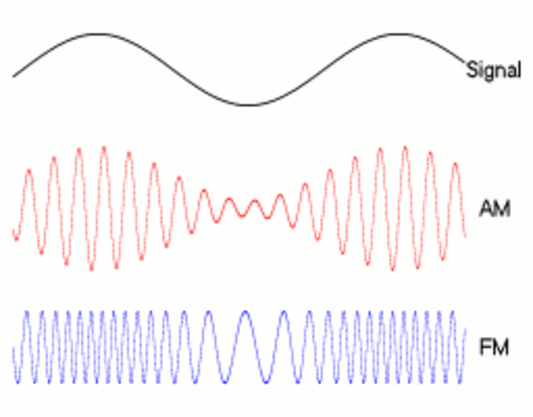
\includegraphics[scale=0.4]{Frequenzaufbereitung/Bilder/Amfm3-en-de.pdf}
% \vspace{-6cm}
%\end{wrapfigure}

\section*{Theorie- und Prüfungsfragen} 


\mucho{1}{TG103}
{Das Blockschaltbild stellt einen Mehrbandsender dar. Welche Frequenz entsteht am Ausgang X, wenn der VFO auf 3,51 MHz eingestellt ist\\ 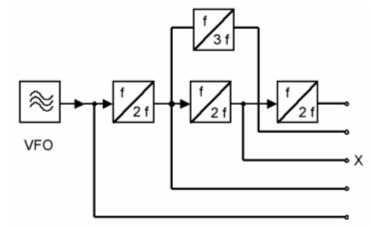
\includegraphics[scale=0.4]{Frequenzaufbereitung/Bilder/TG103a.png}}%Frage
{3,55 MHz}%A
{7,02 MHz}%B
{21,06 MHz}%C
{14,04 MHz}%D
{D}%Lösung

\mucho{2}{TG105}
{Welche Schaltungen sind bei den Stufen  ``A'' und  ``B''  des dargestellten Senders erforderlich?\\ 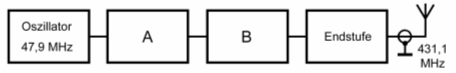
\includegraphics[scale=0.4]{Frequenzaufbereitung/Bilder/TG105.png}}%Frage
{Je ein Frequenzverdreifacher.}%A
{Ein Frequenzverdreifacher und ein Frequenzverdoppler.}%B
{Ein Frequenzvervierfacher und ein Frequenzverdoppler.}%C
{Ein Oberwellenmischer und eine Treiberstufe.}%D
{A}%Lösung

\mucho{3}{TF304}
{Welches sind die wichtigsten Ausgangsfrequenzen, die bei der Mischung einer Frequenz von 30 MHz mit einer Frequenz von 39 MHz entstehen?}%Frage
{39 MHz und 69 MHz}%A
{9 MHz und 39 MHz}%B
{30 MHz und 39 MHz}%C
{9 MHz und 69 MHz}%D
{D}%Lösung

\mucho{4}{TG226}
{Welche wesentlichen Ausgangsfrequenzen erzeugt die in der Abbildung dargestellte Stufe?\\ 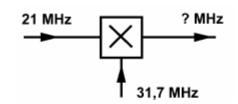
\includegraphics[scale=0.4]{Frequenzaufbereitung/Bilder/TG226.png}}%Frage
{21,4 und 105,4 MHz}%A
{42 und 63,4 MHz}%B
{21 und 63,4 MHz}%C
{10,7 und 52,7 MHz}%D
{D}%Lösung

\mucho{5}{TG101}
{Dieses Blockschaltbild zeigt einen SSB-Sender. Welche Stufe muss beim ? arbeiten?\\ 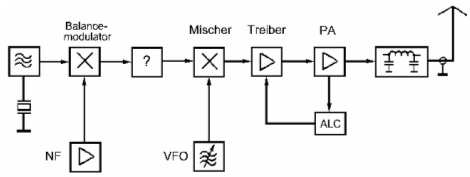
\includegraphics[scale=0.4]{Frequenzaufbereitung/Bilder/TG101.png}}%Frage
{Ein ZF-Notchfilter als Seitenbandsperre.}%A
{Ein USB-Hochpass als Trägerfrequenzsperre.}%B
{Ein LSB-Tiefpass als Trägerfrequenzsperre.}%C
{Ein Quarzfilter als Seitenbandsperre.}%D
{D}%Lösung

\mucho{6}{TD701}
{Welche der nachfolgenden Aussagen ist richtig, wenn die im Bild dargestellte Regelschleife in stabilem Zustand ist?\\ 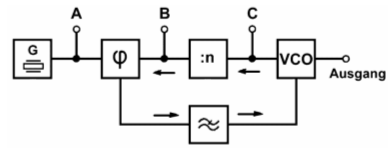
\includegraphics[scale=0.4]{Frequenzaufbereitung/Bilder/TD701.png}}%Frage
{Die Frequenz an Punkt A ist höher als die Frequenz an Punkt B.}%A
{Die Frequenzen an den Punkten A und B sind gleich.}%B
{Die Frequenzen an den Punkten A und C sind gleich.}%C
{Die Frequenz an Punkt B ist höher als die Frequenz an Punkt C.}%D
{B}%Lösung

\mucho{7}{TG110}
{Im folgenden Blockschaltbild ist die Frequenzaufbereitung für einen Amateurfunk-Transceiver dargestellt.\\ 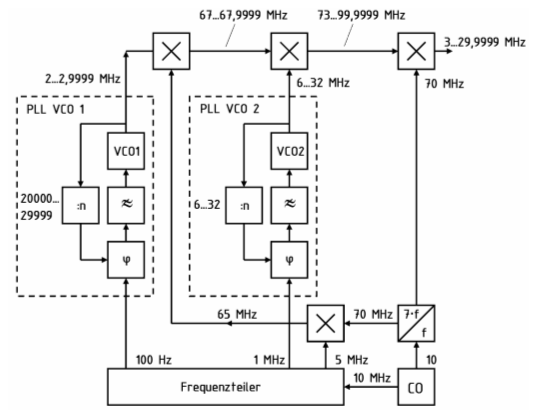
\includegraphics[scale=0.4]{Frequenzaufbereitung/Bilder/TG110.png}\\
Welche Frequenz erzeugt der Sender, wenn VCO1 auf 2,651 MHz eingestellt und VCO2 auf 6 MHz eingerastet ist?}%Frage
{6,651 MHz}%A
{3,651 MHz}%B
{8,651 MHz}%C
{14,351 MHz}%D
{B}%Lösung
